\documentclass[tikz,border=5pt]{standalone}
\usetikzlibrary{shapes.misc, positioning, decorations.pathreplacing, calc}

\newcommand{\particle}[5]{
  \node[draw, align = center,
    anchor = #3,
    minimum height = 1.0cm,
    text width = 1.5cm]
  (#1) at (#2)[draw, rounded rectangle]{$#4$\\\tiny#5};
}
\newcommand{\boson}[5]{
  \node[draw, align = center,
    anchor = #3,
    minimum height = 1.5cm,
    text width = 1.5cm]
  (#1) at (#2)[draw, rounded rectangle]{$#4$\\\tiny#5};
}
\def\shft{5mm}
\def\sep{10mm}
\usepackage{tikz}
\begin{document}
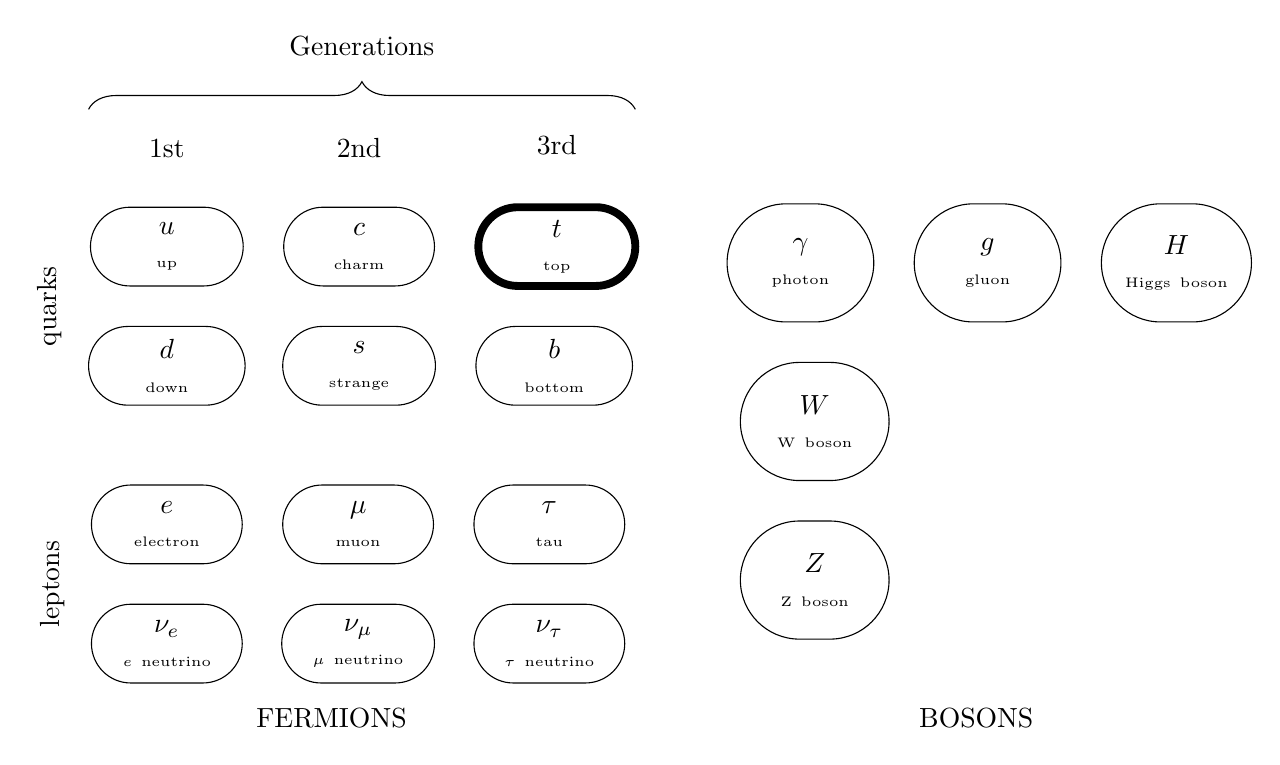
\begin{tikzpicture}
  \begin{scope}[local bounding box=fermions]
    \begin{scope}[local bounding box=quarks]
      \particle{u}{0,0}{center}{u}{up}
      \particle{d}{$(u.south) + (0.0, -\shft)$}{north}{d}{down}
      \particle{c}{$(u.east) + (\shft, 0.0)$}{west}{c}{charm}
      \particle{s}{$(c.south) + (0.0, -\shft)$}{north}{s}{strange}
      \node [align = center,
        anchor = west,
        minimum height = 1.0cm,
        text width = 1.5cm]
      (t) at ($(c.east) + (\shft, 0.0)$)[draw, line width=1mm, rounded rectangle]{$t$\\\tiny top};
      \particle{b}{$(s.east) + (\shft, 0.0)$}{west}{b}{bottom}
    \end{scope}
    \begin{scope}[local bounding box=leptons]
      \particle{e}{$(d.south) + (0.0, -\sep)$}{north}{e}{electron}
      \particle{nue}{$(e.south) + (0.0, -\shft)$}{north}{\nu_{e}}{$e$ neutrino}
      \particle{mu}{$(e.east) + (\shft, 0.0)$}{west}{\mu}{muon}
      \particle{numu}{$(mu.south) + (0.0, -\shft)$}{north}{\nu_{\mu}}{$\mu$ neutrino}
      \particle{tau}{$(mu.east) + (\shft, 0.0)$}{west}{\tau}{tau}
      \particle{nutau}{$(tau.south) + (0.0, -\shft)$}{north}{\nu_{\tau}}{$\tau$ neutrino}
    \end{scope}

    \node [anchor = south](firstgen) at ($(u.north) + (0.0, \shft)$){1st};
    \node [anchor = south](scndgen) at ($(c.north) + (0.0, \shft)$){2nd};
    \node [anchor = south](thrdgen) at ($(t.north) + (0.0, \shft)$){3rd};
    \node [anchor = center](q) at ($(quarks.west) + (-\shft, 0.0)$)[rotate=-270]{quarks};
    \node [anchor = center](q) at ($(leptons.west) + (-\shft, 0.0)$)[rotate=-270]{leptons};
    \draw[decorate, decoration={brace, amplitude=10pt,}]
    ($(quarks.west) + (0.0, 25mm)$) -- ($(quarks.east) + (0.0, 25mm)$) node [midway, yshift=0.8cm] {Generations};
  \end{scope}
  \node(fermionstitle) at ($(fermions.south) + (0.0, -0.2)$)[anchor=north]{FERMIONS};
  \begin{scope}[local bounding box = bosons]
    \boson{photon}{$(t.east |- t.north) + (\sep, 0.0) + 0.5*($(t.east |- t.north) - (t.west |- t.north)$)$}{north}{\gamma}{photon}
    \boson{W}{$(photon.south east) + (0.0, -\shft)$}{north}{W}{W boson} 
    \boson{Z}{$(W.south) + (0.0, -\shft)$}{north}{Z}{Z boson} 
    \boson{gluon}{$(photon.east) + (\shft, 0.0)$}{west}{g}{gluon} 
    \boson{H}{$(gluon.east) + (\shft, 0.0)$}{west}{H}{Higgs boson}
  \end{scope}
  \node(bosonstitle) at ($(fermions.south east) + (\sep, 0.0) + (0.0, -0.2) + 0.5*($(bosons.east) - (bosons.west)$)$)[anchor=north]{BOSONS};
  %\coordinate (D) at  ();
  %\node [align=center](a) [draw, rectangle]{a};
  %\node [align=center, anchor = north](b) at ($(a.south) + (0, -0.3)$) [draw, rectangle]{b};
  %\node [align=center, anchor = west, minimum height=0.5cm, minimum width=0.5cm](c) at ($(a.east) + (0.3, 0)$) \element{c};

\end{tikzpicture}
\end{document}
